\chapter{Magnitudes eléctricas}

En este capítulo, arribaremos a definir \textbf{intensidad de corriente eléctrica}, \textbf{tensión eléctrica}, \textbf{resistencia eléctrica}, y veremos cómo estas tres magnitudes se encuentran relacionadas. Para ello, será necesario contar con nociones acerca de los átomos y su estructura. Tranquilo... no nos detendremos demasiado en estas ideas, pero debés saber que son fundamentales para poder construir una base sólida en la comprensión de los fenómenos eléctricos.

\section{El átomo}

La materia está constituida por unidades muy pequeñas (del orden de los picómetros) llamadas \textbf{átomos}.

Para tener una noción más clara de la pequeñez de los átomos, \textit{el diámetro de un átomo es al diámetro de una manzana como el diámetro de una manzana es al diámetro de la Tierra}.

A su vez, estos átomos poseen un \textbf{núcleo}, formado por \textbf{protones} y \textbf{neutrones}, y uno o varios \textbf{electrones}; todos atraídos o repelidos por lo que se conoce con el nombre de \textbf{fuerza eléctrica}.

Si en el Universo, todas las partículas se atrayeran entre sí, entonces toda la materia estaría comprimida en un único bloque compacto.

Si, por el contrario, todas las partículas se repelieran, el Universo sería un gas en permanente expansión.

Es lógico pensar entonces, que estos tres tipos de partículas (protones, neutrones y electrones), se encuentren atraídas o repelidas entre sí de manera equilibrada para que el Universo pueda subsistir tal y como lo conocemos.

Se dice que los protones tienen carga eléctrica positiva, que repele cargas positivas pero que atrae cargas negativas. Entonces, estos protones positivos en el núcleo, atraen a una nube de electrones negativos a su alrededor para constituir el átomo.

Los electrones, con carga negativa, son atraídos por el núcleo positivo de protones, pero se rechazan entre sí. Son muy ligeros y se mueven muy rápido. 

Debido a este rechazo entre los electrones, no atravesamos una pared al tocarla, ya que los electrones de nuestra mano rechazan a los electrones de la pared.

Si bien la masa de un protón es mucho mayor a la de un electrón, ambos poseen la misma cantidad de carga eléctrica (es decir que un electrón es tan negativo como positivo es un protón). 

Las fuerzas eléctricas de atracción y repulsión, harán que las cargas de un átomo se encuentren balanceadas. En otras palabras: un átomo tendrá la misma cantidad de protones que de electrones, y entonces es eléctricamente neutro.

Aunque los átomos tengan carga neutra, es posible que los electrones de sus capas externas, sean atraídos por el núcleo de otros átomos, provocando una ``asociación" que da lugar a la formación de moléculas.

\subsection{Fuerza eléctrica}

Según la cantidad de electrones que se encuentren atraídos al núcleo de un átomo, se organizarán en diferentes capas o niveles de energía. Mientras la distancia al núcleo sea mayor, la \textbf{fuerza eléctrica} será menor.

La fuerza eléctrica es una magnitud vectorial, que aparece entre dos cuerpos cargados eléctricamente, y puede ser de atracción o de repulsión.

Para comprender mejor la fuerza eléctrica, puede recurrirse a una analogía con la fuerza magnética: 
A medida que se acerca un imán fijo a un metal, se puede percibir que la fuerza de atracción entre ambas piezas es mayor, y a medida que se aleja, la fuerza es menor.

La fuerza eléctrica entre dos cuerpos cargados se calcula mediante la Ley de Coulomb:

$$ F = k \times \frac{q_1 \times q_2}{d^{2}} $$

\begin{itemize}
	\item $k=9 \times 10^{9}\frac{N.m^{2}}{C^{2}}$
	\item $q_1$ y $q_2$ son las cantidades de carga de ambos cuerpos, expresados en Coulombs.
	\item $d$ es la distancia que separa ambos cuerpos.
\end{itemize}

Con respecto a la unidad de carga, \textit{1 Coulomb} equivale a aproximadamente $6,241509\times 10^{18}$ electrones, o $6,24$ millones de billones de electrones... que si bien es una cantidad enorme, sólo representa a la carga que pasa por un cargador de teléfono celular durante unos pocos segundos.

\subsection{Materiales conductores y aislantes}

Aplicando esta Ley, puede deducirse que los electrones de un átomo pueden estar fuerte o débilmente atraídos por el núcleo según la distancia que mantengan con respecto al núcleo.

Si la atracción entre el núcleo y alguno de sus electrones es débil, ese material es conductor. Si, por el contrario, todos los electrones del átomo se encuentran fuertemente atraídos por el núcleo, no se podrán desprender con facilidad del átomo y por lo tanto son materiales aislantes.

Pero la atracción de los electrones con los núcleos de sus respectivos átomos no depende sólo de su ``cercanía al núcleo" sino también de la completud de las capas: los átomos con capas completas suelen ser estables y los átomos con capas incompletas suelen tener más facilidad para ceder electrones (recordando que un material que cede electrones con facilidad es un conductor).

Una capa de electrones puede contener hasta $2n^{2}$ electrones, donde $n$ es el número de capa.

Tomando como ejemplo el cobre, cuyos átomos poseen 29 protones y 29 electrones, los electrones se encuentran distribuidos de la siguiente forma:
\begin{itemize}
	\item Capa 1: 2
	\item Capa 2: 8
	\item Capa 3: 18
	\item Capa 4: 1
\end{itemize}

El electrón de la cuarta capa, se encuentra alejado del núcleo, y además, está en una capa incompleta, porque la cuarta capa puede contener hasta $2\times 4^{2}=32$ electrones, y por estos motivos el cobre es buen conductor de corriente eléctrica.

Si hubiera, en las inmediaciones del átomo de cobre, una fuerza de atracción lo suficientemente fuerte, el electrón de la cuarta capa se liberaría del átomo padre, quedando el átomo con 29 protones y 28 electrones y carga positiva. Cuando esto ocurre, el átomo se convierte en un ion positivo.

\section{Diferencia de potencial eléctrico o tensión}

Algo similar ocurre en todas las baterías: una separación de cargas positivas y cargas negativas, a través de medios químicos.

Una fuente de tensión no es más que un dispositivo con regiones de carga positiva y carga negativa. Mientras mayores sean estas cargas, mayor será la tensión o voltaje.

Para efectuar este proceso de separación de cargas, es necesario gastar cierta energía. Así, la \textbf{diferencia de potencial} se define como el trabajo necesario para mover estas cargas.

\begin{equation} \label{eq:1}
  \text{Dif. de potencial eléctrico } \textbf{ V} = \frac{\text{energía potencial }\textbf{ W}}{\text{carga }\textbf{ Q}}
\end{equation}


Si utilizamos las unidades del S.I., se dice que \textit{1 Volt de potencial equivale a 1 Joule de de energía por 1 Coulomb de carga}

$$ 1 V = 1 \frac{J}{C} $$

\begin{ejemplo}
	Determinar la tensión entre dos puntos si se requieren 80 J de energía para mover 20 C de carga.
	
	\emph{Solución:} Aplicando la ecuación \ref{eq:1}, se tiene $$ \frac{80J}{20C}=4V $$.
\end{ejemplo}

\begin{ejemplo}
	Determinar la energía consumida para mover una carga de 0,05 C entre dos puntos si la tensión entre los mismos es de 10 V.
	
	\emph{Solución:} De la ecuación \ref{eq:1}, se despeja $$ \text{Energía potencial} = \text{Potencial eléctrico} \times \text{carga} $$
	
	Luego $$ 0,05C \times 10V = 0,5 J $$
\end{ejemplo}

\section{Intensidad de corriente eléctrica}

La corriente eléctrica o intensidad de corriente eléctrica, es el flujo de cargas eléctricas; es decir, el movimiento de electrones a lo largo del tiempo.

\begin{equation}
\label{eq:2}
	I=\frac{Q}{t}
\end{equation}

La unidad que utilizamos para la corriente es el Ampere, y equivale a 1 Coulomb de carga fluyendo durante 1 segundo de tiempo:

$$ 1A = \frac{1C}{1s} $$

\begin{ejemplo}
	Determinar la corriente eléctrica en Amperes si la carga que fluye es de 0,01 C durante 5 mS.
	
	\emph{Solución:} De la ecuación \ref{eq:2} se sabe que las unidades deberán ser Coulomb para las cargas y segundos para el tiempo. Por ello, debe realizarse la conversión $5mS=\frac{5}{1000} S =0,005 S$, y a continuación, aplicar la ecuación, obteniendo: $$ I= \frac{0,01 C}{0,005 S} = 2 A $$
\end{ejemplo}

\begin{ejemplo}
	Calcular cuánto tiempo deberá pasar para que circule 1 C de carga si la corriente en un circuito es de 0,3 A.
	
	\emph{Solución:} De la ecuación \ref{eq:2} se despeja el tiempo, obteniendo: 
	\begin{equation}
		\label{eq:3}
		t=\frac{Q}{I}
	\end{equation}
	Y luego, es inmediato que $$ t=\frac{1C}{0,3A}=(1/3)S \approx 0,333 S $$
\end{ejemplo}

\section{Relación entre tensión y corriente: la resistencia}

Es común confundir tensión con corriente, pero son dos términos completamente diferentes.

Aplicar una tensión a un material conductor hará que fluya corriente eléctrica por el mismo.

La tensión es la causa, mientras que la corriente es la consecuencia.

Sin tensión no puede haber corriente eléctrica, pero sí puede existir tensión entre dos puntos sin una corriente que circule entre los mismos (esto ocurre, por ejemplo, entre los bornes de una pila que no está conectada en un circuito, ya que existe tensión pero no hay corriente circulando entre los mismos).

Si la tensión es la causa de la corriente, evidentemente una modificación de los valores de tensión alterará la corriente obtenida.

La \textbf{resistencia} es la medida de la oposición que presenta un determinado material al paso de la corriente eléctrica. Para medirla, se utiliza como unidad el \textbf{Ohmio}, que se simboliza con la letra griega $\Omega$ .
\subsection{Ley de Ohm}
Si se piensa en una definición del tipo $ \textit{Efecto} = \frac{\textit{Causa}}{\textit{Oposición}}$, se puede definir la \textbf{Ley de Ohm} como sigue:

\begin{equation}
	\label{eq:ohm_i}
	I=\frac{V}{R}
\end{equation}
donde $V$ es la tensión en Voltios, $I$ es la intensidad de corriente en Amperes y $R$ es la resistencia en ohmios.

\begin{figure}[h]
	\label{gr:ohm}
	\caption{Circuito básico}
	
%	\begin{pspicture}(0,0)(6,5)
%
%		\pnodes(1,1){A}(1,4){B}(5,1){C}(5,4){D}
%		\vdc(B)(A){$V$}
%		\resistor[dipolestyle=zigzag, tensionlabel=$I$](C)(D){$R$}
%
%		\wire(A)(C)
%		\wire(B)(D)
%	\end{pspicture}

\end{figure}

De la ecuación \ref{eq:ohm_i} se pueden despejar:
\begin{equation}
	\label{eq:ohm_v}
	V=I \times R
\end{equation}
\begin{equation}
	\label{eq:ohm_r}
	R=\frac{V}{I}
\end{equation}
\section{Potencia (para corriente continua)}
La \textbf{potencia} es la cantidad de trabajo que puede realizarse en una cantidad de tiempo. En otras palabras, es \textit{la velocidad a la que se realiza un trabajo}.

\begin{ejemplo}
	Un motor GRANDE posee más potencia que un motor PEQUEÑO porque puede realizar más trabajo en la misma cantidad de tiempo.
\end{ejemplo}

En términos analíticos, la potencia (en Watts o vatios) es la relación entre trabajo (en Joules) y tiempo (en segundos).

\begin{equation}
	\label{eq:pot}
	P = \frac{W}{t}
\end{equation}

Despejando $W$ en la ecuación \ref{eq:1}, se obtiene $ W=QV $. Esto puede aplicarse en la ecuación \ref{eq:pot}, obteniendo:

$$ P =\frac{QV}{t}=V\frac{Q}{t} $$

Finalmente, reemplazando la ecuación de corriente \ref{eq:2} en ésta última, se obtiene:
\begin{equation}
	\label{eq:pot_cc1}
	P = V \times I
\end{equation}

También puede reemplazarse esta última ecuación en la Ley de Ohm, obteniendo:

\begin{equation}
	\label{eq:pot_cc2}
	P = \frac{V^{2}}{R}
\end{equation}

\begin{equation}
	\label{eq:pot_cc3}
	P = I^{2}R
\end{equation}

\subsection{Energía}

Para que la potencia convierta energía de cualquier forma, se debe utilizar durante un tiempo. Cuanto más tiempo se consuma la potencia, mayor será la energía consumida.

\begin{equation}
	\label{eq:w}
	W=P\times t \text{ energía en Watts/hora}
\end{equation}

\begin{equation}
	\label{eq:w_kwh}
	W=P\times t \times 1/1000 \text{ energía en kiloWatts/hora}
\end{equation}
La energía $W$ se medirá en $Wh$ (watts/hora) o $kWh$ (kilowatts/hora) según convenga.

Nótese que la unidad para el tiempo establecida por el SI es el segundo, pero en este caso resulta muy pequeño (y por lo tanto los valores medidos usando esta unidad serían muy grandes), y debe tenerse especial cuidado al operar con estas magnitudes, ya que puede ser necesario realizar conversiones.

\subsection{Eficiencia}

La eficiencia $\eta$ (eta) se define como la relación entre la \textbf{potencia de entrada} y la \textbf{potencia de salida} del sistema.
\begin{equation}
	\label{eq:efi}
	\eta = \frac{P_{salida}}{P_{entrada}}
\end{equation}

Este es un valor decimal que varía entre 0 y 1. Habitualmente, se lo suele expresar en porcentaje (por lo que se debería multiplicar la expresión anterior por 100)

\begin{equation}
	\label{eq:efiporc}
	\eta \% = \frac{P_{salida}}{P_{entrada}} \times 100
\end{equation}

Si la eficiencia de un sistema fuera del 100$\%$, esto significaría que su potencia de entrada es igual a la potencia de entrada. En la práctica, sabemos que esto no es posible, porque todo sistema tendrá pérdidas por transformación de energía, y esto implica una diferencia entre las potencias: $$ P_{entrada} = P_{salida} + P_{perdida} $$ 

\section{Campos eléctricos}

Alrededor de un cuerpo cargado, existirá un \textbf{campo eléctrico}. A medida que la distancia al cuerpo sea menor, la \textbf{densidad del campo eléctrico} será mayor.

La \textbf{densidad de flujo } se define como la relación entre las líneas de flujo y el área que se está evaluando. Como la densidad de carga aumenta consecuentemente con la carga eléctrica, ambas magnitudes (carga y flujo) pueden igualarse. $$ \text{Densidad} = \frac{\text{Carga}}{\text{Área}} $$

La \textbf{fuerza del campo eléctrico} $F_{ce}$ es la fuerza que actúa sobre una carga Q en un punto:
$$ F_{ce} = \frac{F}{Q} $$

Reemplazando la fuerza en la ecuación anterior según la \textit{Ley de Coulomb}, se obtiene: 
\begin{equation}
	\label{eq:fuerza_electrica_capacitor}
	F_{ce} = \frac{kQ}{r^{2}}
\end{equation}


Esto quiere decir, que la fuerza del campo eléctrico está relacionada con el tamaño de la carga y la distancia que se mantenga con ésta. A medida que la distancia sea mayor, la fuerza eléctrica será \textit{mucho menor} (dado que el término en el denominador está elevado al cuadrado).

\subsection{Capacitores}

Existe un componente electrico cuyo principio de funcionamiento está directamente relacionado con los campos eléctricos: \textbf{el capacitor}.

\subsubsection{Construcción y principio de funcionamiento}

Un capacitor está constituido por dos placas conductoras paralelas separadas a una distancia mínima, por un material \textbf{dieléctrico} (aislante), que puede ser aire, mica, cerámica, poliéster, entre otros.

\begin{figure}[htbp]
  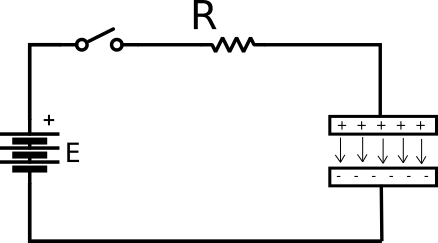
\includegraphics[scale=1]{images/capacitor_circuito_carga}
  \caption{Circuito de carga básico de un capacitor}
  \label{fig:cap_carga}
\end{figure}

Dado el circuito de la figura \ref{fig:cap_carga}, al cerrar el interruptor y por ahora omitiendo la resistencia (o suponiendo que posee una resistencia de $0 \Omega$), la placa inferior se comenzará a cargar con electrones libres, y la placa superior con cargas positivas.

Entre las placas, se alcanzará la tensión de la fuente $E$.

Como la distancia entre ambas es muy pequeña, las cargas se verán atraídas por una fuerza eléctrica (que recordando la ecuación \ref{eq:fuerza_electrica_capacitor}, será mayor si la distancia entre ambas es menor), y permanecerán atraídas incluso si se elimina la fuente de alimentación (o si se abre el circuito con el interruptor).

\begin{figure}[htbp]
  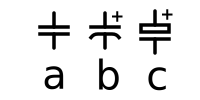
\includegraphics[scale=1]{images/capacitor_simbolo}
  \caption{Símbolos del capacitor: (a) No polarizado, (b) y (c) Polarizado}
  \label{fig:cap_simbolos}
\end{figure}

\subsubsection{Capacitancia}

La \textbf{capacitancia} de un capacitor es la cantidad de cargas que puede almacenar en él, cuando está completamente cargado.

\begin{equation}
	\label{eq:capacitancia}
	C = \frac{Q}{V}
\end{equation}

La unidad utilizada para medir la capacidad es el \textbf{Farad}, y 1 Farad de carga equivale a una carga de 1 Coulomb a una diferencia de potencial de 1 volt.
$$ 1 \text{Farad} = \frac{1 C}{1 V}$$

Redefiniendo la ecuación \ref{eq:fuerza_electrica_capacitor} para el caso del capacitor, resulta
\begin{equation}
	F_{ce} = \frac{V}{d}
\end{equation}

considerando la fuerza eléctrica en $Voltios/metro$, la tensión en $voltios$ y la distancia en $metros$.

El campo eléctrico también es afectado por la \textbf{permitividad} del material que se utiliza como dieléctrico. Un aumento en la permitividad del material, permitirá que la misma carga se almacene con un campo eléctrico menor; es decir, con un potencial eléctrico menor. Analizando la ecuación \ref{eq:capacitancia}, si la tensión disminuye, la capacitancia aumentará. En otras palabras, \textit{si la permitividad del dieléctrico es mayor, la capacidad será mayor}.

La permitividad $\epsilon $ se define como $ \epsilon = \frac{\epsilon_r}{\epsilon_0}$, donde $\epsilon_r$ es la permitividad relativa del material y $\epsilon_0 $ es la permitividad del vacío.

En la siguiente tabla, se recopilan los valores de algunos materiales utilizados para la construcción de dieléctricos de capacitores.

\begin{tabular}{|c|c|}
\hline 
Material & Permitividad relativa \\ 
\hline 
Aire & 1,0006 \\ 
\hline 
Papel & 1,5 \\ 
\hline 
Aceite & 2,8 \\ 
\hline 
Mica & 4 \\ 
\hline 
Cuarzo & 4,5 \\ 
\hline 
Baquelita & 5 \\ 
\hline 
PVC & 30 a 40 \\ 
\hline 
Agua destilada & 80 \\ 
\hline 
Acetona & 191 \\ 
\hline 
\end{tabular} 

Si se desea calcular la capacitancia teniendo en cuenta los valores de permitividad eléctrica, la ecuación es la siguiente,

\begin{equation}
	\label{eq:capacitancia_permitividad}
	C = \epsilon \frac{A}{d}
\end{equation}

considerando $\epsilon $ en $Farad/metro$, el área en metros cuadrados, la distancia en metros y la capacidad en Farads.

Debe tenerse en cuenta que los capacitores poseen un \textbf{voltaje de trabajo máximo}, que representa la máxima tensión que puede aplicarse en forma continua sin dañar el dispositivo. Si se excede, se puede dañar el dieléctrico.

\section{Campos magnéticos}

Alrededor de un imán permanente existe un campo magnético. Así como se usaron líneas de campo eléctrico para representar los efectos de un campo eléctrico, se usarán \textbf{líneas de flujo magnético} para describir el comportamiento de los campos magnéticos.

Las líneas de flujo irradian del polo norte al polo sur del imán, y regresan al norte por el interior del mismo.

Si el imán se divide, aparecerán nuevos polos norte y sur en cada material.

Como se sabe popularmente, los polos opuestos de los imanes generan una fuerza de atracción, mientras que los polos semejantes se repelerán.

Los materiales en los cuales es posible establecer con facilidad líneas de flujo magnético son \textbf{ferromagnéticos}, mientras que aquellos que provocan más dificultad para esta tarea son \textbf{diamagnéticos}. La magnitud que distingue esta propiedad (el magnetismo) de un material, es la \textbf{permeabilidad} y se simboliza con $\mu$.

Si un material \textbf{diamagnético} se interpone en un campo magnético, no le provocará una interferencia demasiado grande, y el campo lo atravesará, casi como si este material no estuviera. Si, por el contrario, se interpone un material \textbf{ferromagnético}, el campo pasará por el material en vez de por el aire, modificando la trayectoria de las líneas de flujo.

Alrededor de todo conductor por el que circule una corriente, existirá un campo magnético.

\begin{figure}
	
	\centering
		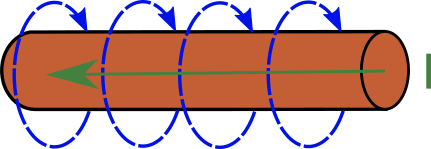
\includegraphics[scale=0.5]{images/electroiman-un-hilo}

	\caption{\label{fig:electroiman-hilo} Sentido de la corriente y del campo magnético en conductor de un hilo}
\end{figure}

Si es un conductor como el de la figura \ref{fig:electroiman-hilo}, aparecerá un campo magnético, con líneas de flujo en el sentido mostrado por las líneas azules.

\begin{figure}
	\centering
		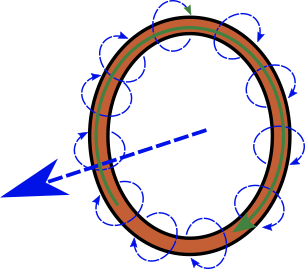
\includegraphics[scale=0.5]{images/electroiman-espira}
	
	\caption{\label{fig:electroiman-espira} Sentido de la corriente y del campo magnético en una espira}
\end{figure}
Si, en cambio, el conductor es una espira como la de la figura~\ref{fig:electroiman-espira}, el campo resultará en una dirección común, como muestra la flecha azul gruesa.

\begin{figure}
	\centering
		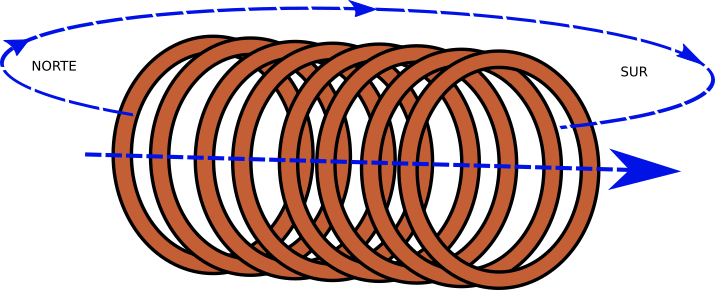
\includegraphics[scale=0.5]{images/electroiman-bobina}
	\caption{\label{fig:electroiman-bobina} Sentido de la corriente y del campo magnético en una bobina}
\end{figure}
Finalmente, por un bobinado (más de una vuelta), como el de la figura ~\ref{fig:electroiman-bobina}, se producirá un campo magnético de trayectoria continua, muy parecida a la de un imán permanente.
Este es el principio de funcionamiento del electroimán.

La cantidad de líneas de flujo por área unitaria se denomina \textbf{densidad de flujo},

\begin{equation}
	\label{eq:densidad_flujo}
	B = \frac{\Phi}{A}
\end{equation}

Siendo las unidades utilizadas en el Sistema Internacional:
\begin{itemize}
	\item Teslas ($T$) para la densidad,
	\item Weber ($Wb$) para el flujo magnético y
	\item Metros cuadrados ($m^{2}$) para el área.
\end{itemize}

La densidad de flujo en un electroimán se relaciona de manera directa con el número de vueltas del bobinado ($N$) y la corriente que lo atraviesa ($I$). Estas dos magnitudes se relacionan dando lugar a la \textbf{fuerza magnetomotriz}:
\begin{equation}
	\label{eq:fuerza_magnetomotriz}
	F_{m} = N \times I
\end{equation}

\subsection{Inductores}

El dispositivo descrito en la sección anterior se llama \textbf{inductor}, y consiste simplemente en un bobinado por el cual se hace circular una corriente eléctrica.

La fuerza del campo magnético es determinada por la \textbf{inductancia} del inductor.

La inductancia es la medida de la oposición a un cambio de corriente en el inductor y se mide en Henries ($H$).

Existen varios factores que intervienen en los valores de inductancia:
\begin{itemize}
	\item Permeabilidad del material del núcleo $\mu$ ($Wb/A\times m$).
	\item Cantidad de vueltas del devanado N.
	\item Área A ($m^{2}$).
	\item Longitud l ($m$).
\end{itemize}

Todos estos valores se relacionan en la siguiente ecuación:
\begin{equation}
	\label{eq:inductancia}
	L= \frac{\mu N^{2}A}{l}
\end{equation}
\section{Sobre la resistencia, capacidad e inductancia}
Cuando se observa un circuito con un símbolo de resistencia, se piensa inmediatamente en el componente eléctrico resistor. De igual manera, ocurre al observar los símbolos de capacitor e inductor. En muchos casos, estos símbolos se utilizan para representar otros elementos que consuman o absorban energía. Por ejemplo, una resistencia puede ser un calefactor o una lámpara, o un inductor podría ser un parlante o un motor.

La inductancia aparecerá alrededor de cualquier conductor por el cual circule corriente eléctrica
En los capítulos siguientes, se trabajará brevemente con estas magnitudes, para poder analizar su comportamiento transitorio y en frecuencia, que es donde surgen sus propiedades más interesantes.